\documentclass[12pt,a4paper]{article}
\usepackage[utf8]{inputenc}
\usepackage{polski}
\usepackage[polish]{babel}
\usepackage{amsmath}
\usepackage{amsfonts}
\usepackage{amssymb}
\usepackage{graphicx}
\usepackage[export]{adjustbox}
\usepackage{wrapfig}
\usepackage{caption}

\numberwithin{equation}{section}

\renewcommand{\baselinestretch}{1.5}
\captionsetup[figure]{labelformat={default},name={\bfseries Rys.}}
\captionsetup[table]{labelformat={default},name={\bfseries Tab.}}

\newcommand*{\captionsource}[2]{%
	\caption[{#1}]{%
		#1%
		\\\hspace{\linewidth}%
		\textbf{Żródło:} #2%
	}%
}


\title{0. Opracowanie danych pomiarowych}
\date{11 października 2017}	
\author{
	Zespół 3: Górski Paweł, Sozańska Ada\\
	EAIiIB Informatyka, Rok II
}

\begin{document}
\maketitle
% WPROWADZENIE
\section{Wprowadzenie}
Celem tego doświadczenia jest zaznajomienie się z podstawowymi metodami opracowania danych pomiarowych. W tym celu wykorzystamy wyniki pomiarów wahadła prostego, dzięki którym obliczymy przybliżoną wartość przyspieszenia ziemskiego $g$.

\subsection{Błędy pomiarów}

Błąd pomiaru $b$ rozumiemy jako różnicę między wartościami zmierzoną $x_i$ oraz rzeczywistą $x_0$

\begin{equation}
	b = x_i - x_0.
\end{equation}

W praktyce wartość rzeczywistą utożsamiamy z wynikiem pomiaru wykonanym dokładniejszą metodą.

\pagebreak
Rozróżniamy kilka rodzajów błędów pomiaru, są nimi:
\begin{itemize}
	\item błąd przypadkowy,
	\item błąd systematyczny,
	\item błąd gruby.
\end{itemize}

Błąd przypadkowy charakteryzuje rozrzut wyników pomiaru wokół wartości rzeczywistej. W przybliżeniu występuje taka sama szansa na otrzymanie wyników $x_i$ większych, jak i mniejszych od $x_0$.

O błędzie systematycznym mówimy, gdy występuje taka sama różnica między wartościami zmierzonymi $x_i$ oraz wartością rzeczywistą $x_0$. Rozrzut wyników pomiaru jest niewielki lub nie występuje.

Błąd gruby występuje, gdy między wynikiem pomiaru $x_i$ a wartością rzeczywistą $x_0$ istnieje duża różnica. Ten błąd pojawia się głównie na skutek nieumiejętności użycia danego przyrządu lub pomyłek przy odczytywaniu i zapisie wartości.

\subsection{Niepewności pomiarów}

Niepewność pomiaru jest parametrem związanym z wynikiem pomiaru, charakteryzującym rozrzut wyników. Rozrzut ten można z uzasadnieniem przypisać wartości mierzonej. Rozróżniamy dwie główne niepewności: graniczną $\Delta x$ oraz standardową $u(x)$.

Mając do czynienia z niepewnością graniczną $\Delta x$ staramy się określić przedział, w którym mieszczą się wszystkie wyniki pomiaru $x_i$:
\begin{equation}
	x_0 - \Delta x < x_i < x_0 + \Delta x.
\end{equation}

Najpowszechniej stosowaną miarą dokładności jest niepewność standardowa $u(x)$, będąca oszacowaniem odchylenia standardowego:
\begin{equation}
	u(x) = \sqrt{\frac{\sum_{i = 0}^n(x_i - \bar{x})^2}{n(n-1)}},
	\label{eq:std_uncert}
\end{equation}

gdzie $x_i$ to wartości pomiaru, $\bar{x}$ oznacza średnią arytmetyczną z wyników pomiaru, a $n$ to ilość wartości zmierzonych.

Rozróżniamy również niepewność względną, która ma ścisły związek z niepewnością standardową. Definiowana jest jako stosunek niepewności bezwzględnej $u(x)$ do wielkości mierzonej:
\begin{equation}
	u_r(x) = \frac{u(x)}{x}.
\end{equation}

\subsection{Ocena niepewności typu A}

Mając pomiary, w których występuje błąd przypadkowy, możemy się posłużyć oceną typu A w celu wyznaczenia niepewności tego pomiaru. 

Mając serię $n$ wyników $x_0, \ldots, x_n$, możemy zminimalizować błąd przypadkowy przyjmując za wynik pomiaru $x$ średnią arytmetyczną:
\begin{equation}
	x \equiv \bar{x} = \frac{1}{n}\sum_{i = 0}^{n}x_i
\end{equation}

Jako, że za wynik pomiaru przyjmujemy średnią, niepewnością tego wyniku będzie estymator odchylenia standardowego średniej
\begin{equation}
	u(x) = \frac{s_x}{\sqrt{n}},
	\label{eq:uncert_sx}
\end{equation}
który ilościowo jest $\sqrt{n}$ razy mniejszy od estymatora odchylenia standardowego $s_x$
\begin{equation}
	s_x = \sqrt{\frac{\sum_{i = 0}^n(x_i - \bar{x})^2}{n-1}}.
	\label{eq:sx}
\end{equation}

Łącząc wzory (\ref{eq:uncert_sx}) oraz (\ref{eq:sx}) otrzymujemy wzór (\ref{eq:std_uncert}).

\subsection{Ocena niepewności typu B}

Kiedy statystyczna analiza wyników jest niemożliwa, posługujemy się oceną typu B (np. gdy wartości pomiaru obarczone są błędem systematycznym lub gdy posiadamy tylko jeden rezultat pomiaru). Ocena ta opiera się na naukowym osądzie eksperymentatora wykorzystującym wszystkie informacje o pomiarze i możliwych źródłach niepewności tego pomiaru.

Najczęściej ocena typu B stosowana jest do określenia dokładności przyrządów pomiarowych. Dla prostych przyrządów mechanicznych (suwmiarka, termometr), przyjmujemy za dokładność wartość najmniejszej działki skali zwaną działką elementarną.

Dla przyrządów cyfrowych lub analogowych niepewność pomiaru jest podawana przez producenta w instrukcji przyrządu. Dla urządzeń cyfrowych dokładność definiujemy jako:
\begin{equation}
	\Delta x = C_1 \cdot x + C_2 \cdot zakres,
\end{equation}
gdzie $C_1, C_2$ znajdują się w instrukcji lub na urządzeniu, a $x$ to wartość mierzona.

Dla analogowych urządzeń pomiarowych dokładność definiujemy jako:
\begin{equation}
	\Delta x = \frac{klasa~przyrzadu}{100} \cdot zakres.
\end{equation}
Klasę przyrządu również można znaleźć zaznaczoną na urządzeniu.

Uzyskane niepewności z powyższych wzorów należy zamienić na niepewność standardową:
\begin{equation}
	u(x) = \frac{\Delta x}{\sqrt{3}}.
\end{equation}

\pagebreak
\subsection{Prawo przenoszenia niepewności}
Szacowanie niepewności dla wielkości fizycznych, których nie sposób zmierzyć jednym przyrządem, wyznaczamy metodą pomiaru pośredniego. Przypuśćmy, że interesuje nas wielkość $y$ zależna od zmiennych $x_0, \ldots, x_n$, które da się zmierzyć bezpośrednio. Na mocy prawa przenoszenia niepewności możemy obliczyć niepewność złożoną $y$ korzystając ze wzoru:
\begin{equation}
	u_c(y) = \sqrt{\sum_{i=0}^{n}\Bigg(\frac{\partial y}{\partial x_k}u(x_k)\Bigg)^2}.
	\label{eq:uc}
\end{equation}

Wzór ten można przenieść na funkcję jednej zmiennej:
\begin{equation}
	u_c(y) = \Bigg|\frac{\partial y}{\partial x_k}u(x_k)\Bigg|.
	\label{eq:uc_single}
\end{equation}

Jeżeli mamy do czynienia z niepewnościami względnymi możemy zastosować następujący uproszczony wzór (wynikający ze wzoru \ref{eq:uc}):
\begin{equation}
	\frac{u_c(y)}{y} = \sqrt{\sum_{i=0}^{n}\Bigg(\frac{u(x_k)}{x_k}p_k\Bigg)^2},
\end{equation}
gdzie:
\begin{equation}
	p_k = \frac{x_k}{y} \frac{\partial y}{\partial x_k}.
\end{equation}

Do porównywania wyników pomiaru z innymi rezultatami będziemy wykorzystywać niepewność rozszerzoną. Jest to iloczyn współczynnika rozszerzenia $k$ oraz niepewności złożonej $u_c$:
\begin{equation}
	U(y) = k u_c(y).
	\label{eq:uc_exp}
\end{equation}
Wartość $k$ jest wybierana w taki sposób, aby przeważająca część wyników znalazła się w przedziale $(y - U(y),~y + U(y))$. Najczęściej przyjmujemy wartość $k = 2$, chociaż w uzasadnionych przypadkach może być większa.

Dwa wyniki pomiaru uważamy za zgodne ze sobą, jeżeli prawdziwa jest nierówność:
\begin{equation}
	|y_1 - y_2| < U(y_1 - y_2),
\end{equation}
gdzie $y_1$ oraz $y_2$ to wyniki, które chcemy ze sobą porównać oraz:
\begin{equation}
	U(y_1 - y_2) = k\sqrt{\Big(u(y_1)\Big)^2 + \Big(u(y_2)\Big)^2}.
\end{equation}

\subsection{Wahadło proste}

Wahadło proste to masa punktowa $m$ zawieszona na nieważkiej, nierozciągliwej nitce, oscylująca w jednorodnym polu grawitacyjnym. Do doświadczenia wykorzystany zostanie model (ciężki metalowy cylinder zawieszony na nitce krawieckiej), który traktujemy jako przybliżenie wahadła prostego.

W naszym ćwiczeniu stosujemy aproksymację
\begin{equation}
	\label{eq1}
	\sin x \approx x,
\end{equation}
która jest prawdziwa na mocy twierdzenia Taylora dla odpowiednio małych wartości kąta $x$. Wzór \ref{eq1} upraszcza równanie określające okres drgań $T$ wahadła w zależności od długości nici $l$ oraz przyspieszenia ziemskiego $g$
\begin{equation}
	\label{eq2}
	T = 2\pi\sqrt{\frac{l}{g}}.
\end{equation}

\pagebreak
% WYKONANIE ĆWICZENIA
\section{Wykonanie ćwiczenia}
\begin{wrapfigure}{l}{0.4\textwidth}
	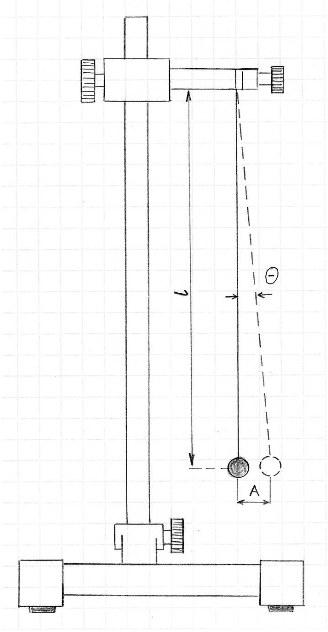
\includegraphics[width=0.4\textwidth]{img/wahadlo.png} 
	\captionsource{Schemat wahadła}{instrukcja do ćw.}
	\label{fig:img1}
\end{wrapfigure}

W celu wykonania doświadczenia wykorzystaliśmy:
\begin{itemize}
	\item Zestaw wahadła prostego (Rys. \ref{fig:img1}),
	\item Sekundomierz (stoper),
	\item Przymiar milimetrowy (linijka 50cm).
\end{itemize}

Doświadczenie rozpoczęliśmy pomiarem ustalonej długości wahadła za pomocą linijki o działce elementarnej 1mm. Osobno mierzone były: długość nici do punktu styku z cylindrem oraz połowa wysokości cylindra. Następnie przy pomocy stopera mierzyliśmy czas 20 okresów wahadła w pojedynczym ruchu (bez zatrzymywania ruchu). Po 5 takich pomiarach wahadło miało już bardzo małą amplitudę drgań, przez co następne 5 pomiarów wykonaliśmy dla nowego ruchu wahadła.

W dalszej części ćwiczenia zmierzyliśmy 20 okresów drgania wahadła dla jego różnych długości. Ze względu na długość nici, wykonaliśmy 10 takich pomiarów. Następnie używając metody regresji liniowej wyznaczyliśmy wartość przyspieszenia ziemskiego $g$.
\pagebreak
% OPRACOWANIE DANYCH POMIAROWYCH
\section{Opracowanie danych pomiarowych}
\subsection{Pomiary}
Zmierzona długość wahadła wynosi $l = 341$ mm. Niepewność pomiaru długości wahadła $l$ wynosi $u(l) = 1$ mm, ponieważ jest to najmniejsza działka elementarna wykorzystanego narzędzia.

\begin{table}[!ht]
	\caption{Wartości pomiarów okresów wahadła dla stałej długości}
	\begin{center}
		\begin{tabular}{r|r|r|r}
			\hline
			\multicolumn{1}{c|}{L.p.} & \multicolumn{1}{c|}{liczba okresów $k$} & \multicolumn{1}{c|}{czas $t$ dla $k$ okresów [s]} & \multicolumn{1}{c}{okres $T_i = t/k$ [s]} \\ \hline \hline
			1 & 20 & 22,61 & 1,130 \\
			2 & 20 & 22,88 & 1,144 \\
			3 & 20 & 22,64 & 1,132 \\
			4 & 20 & 22,78 & 1,139 \\
			5 & 20 & 22,77 & 1,138 \\
			6 & 20 & 22,88 & 1,144 \\
			7 & 20 & 23,09 & 1,154 \\
			8 & 20 & 23,07 & 1,153 \\
			9 & 20 & 23,15 & 1,157 \\
			10 & 20 & 23,24 & 1,162 \\ \hline
		\end{tabular}
	\end{center}
	\label{tab:tab1}
\end{table}
Wartość średnia okresu $T$ dla wyników pomiaru okresu $T_i$ (Tab. \ref{tab:tab1}) jest równa $T = 1,145~\textrm{s}$. 

Korzystając ze wzoru (\ref{eq:std_uncert}) niepewność pomiaru $u(T)$ jest równa
\begin{equation}
	u(T) = \sqrt{\frac{\sum_{i=1}^{10}(T_i - T)^2}{n(n-1)}},
\end{equation}

Dla danych z tabli otrzymujemy wynik $u(T) = 0,0034$ s.

Poniżej znajdują się wyniki pomiarów (Tab. \ref{tab:tab2}) przy zmiennej długości wahadła potrzebne do wykonania regresji liniowej.
\begin{table}[!ht]
	\caption{Wartości pomiarów okresów wahadła dla zmiennej długości}
	\begin{center}
		\begin{tabular}{r|r|r|r|r|r}
			\hline
			\multicolumn{1}{c|}{L.p.} & \multicolumn{1}{c|}{$l$ [mm]} & \multicolumn{1}{c|}{k} & \multicolumn{1}{c|}{$t$ [s]} & \multicolumn{1}{c|}{$T_i$ [s]} & \multicolumn{1}{c}{$T_{i}^{2} ~[\textrm{s}^2]$} \\ \hline \hline
			1 & 439 & 20 & 26,2 & 1,310 & 1,716 \\
			2 & 403 & 20 & 24,9 & 1,245 & 1,550 \\
			3 & 366 & 20 & 23,68 & 1,184 & 1,401 \\
			4 & 327 & 20 & 22,55 & 1,127 & 1,270 \\
			5 & 285 & 20 & 21,16 & 1,058 & 1,119\\
			6 & 241 & 20 & 19,32 & 0,9660 & 0,9331 \\
			7 & 194 & 20 & 17,87 & 0,8935 & 0,7983 \\
			8 & 153 & 20 & 15,19 & 0,7595 & 0,5768 \\
			9 & 108 & 20 & 13,21 & 0,6605 & 0,4362 \\
			10 & 63 & 20 & 10,34 & 0,5170 & 0,2672 \\ \hline
		\end{tabular}
	\end{center}
	\label{tab:tab2}
\end{table}

\pagebreak
\subsection{Analiza wyniku dla stałej długości wahadła}
Wartość przyspieszenia ziemskiego $g$ dla długości wahadła $l$ oraz okresu wahadła $T$ wynosi:
\begin{equation}
	\begin{split}
		&l = 0,341~\textrm{m},~~T = 1,145~\textrm{s}, \\ 
		&g = 4\pi^2\frac{l}{T^2} \approx 10,26~\frac{\textrm{m}}{\textrm{s}^2}.
	\end{split}
\end{equation}

Korzystając ze wzoru (\ref{eq:uc}) na niepewność złożoną otrzymujemy:
\begin{equation}
	\begin{split}
	u_c(g) & = \sqrt{\Bigg(\frac{4\pi^2}{T^2}u(l)\Bigg)^2 + \Bigg(-8\pi^2\frac{l}{T^3}u(T)\Bigg)^2} \\
	 	   & \approx \sqrt{9,06 \cdot 10^{-4} + 37,82 \cdot 10^{-4}} \\ & \approx0,068~\Big[\frac{\textrm{m}}{\textrm{s}^2}\Big]
	\end{split}
\end{equation}

Niepewność złożona $u_c(g)$ oraz niepewność rozszerzona $U(g)$ (wzór \ref{eq:uc_exp}) wynoszą:
\begin{align}
	u_c(g) = 0,068~\frac{\textrm{m}}{\textrm{s}^2},\\
	U(g) = 0,136~\frac{\textrm{m}}{\textrm{s}^2}.
\end{align}

Wartość tabelaryczna przyspieszenia ziemskiego w Krakowie wynosi $g_0 = 9,811~\frac{\textrm{m}}{\textrm{s}^2}$.

\begin{equation}
	|g - g_0| = 0,37 > U(g) = 0,136~\Big[\frac{\textrm{m}}{\textrm{s}^2}\Big]
	\label{eq:gconst}
\end{equation}

Wynik wskazuje na to, że mógł zostać popełniony błąd systematyczny podczas pomiarów okresów wahadła (żadne dane nie odbiegają od siebie w znaczący sposób). Prawdopodobnie wynika on z braku synchronizacji osób przeprowadzających doświadczenie.

\pagebreak
\subsection{Analiza wyniku dla zmiennej długości wahadła}
\begin{figure}[!ht]
	\centering
	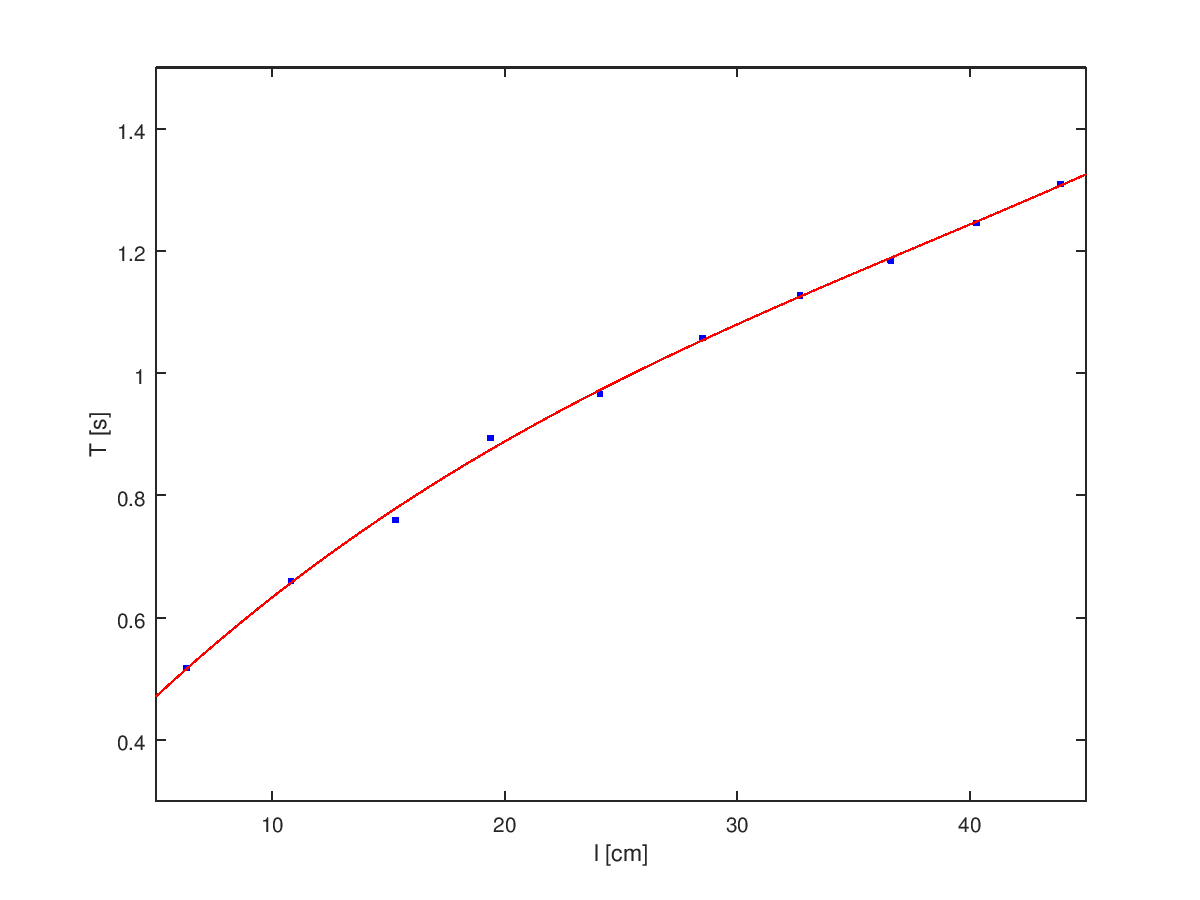
\includegraphics[width=\textwidth]{img/plot1.png} 
	\caption{Wykres zależności okresu od długości wahadła}
	\label{fig:img2}
\end{figure}

Na wykresie (Rys. \ref{fig:img2}) widzimy funkcję okresu wahadła od jego długości. Punkty leżą na krzywej pierwiastkowej, co widać na wykresie zależności $T^2(l)$ znajdującym się poniżej (Rys. \ref{fig:img3}).


\begin{figure}[!ht]
	\centering
	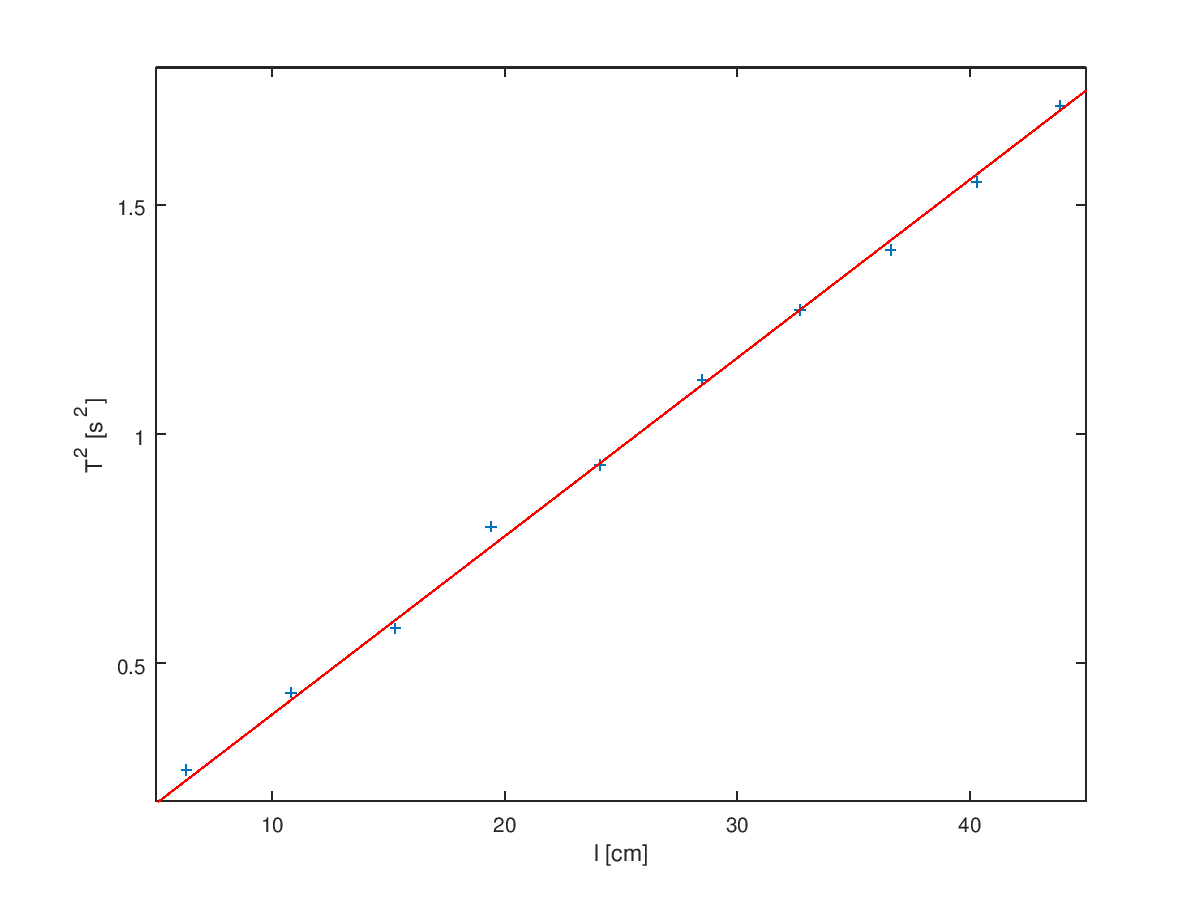
\includegraphics[width=\textwidth]{img/plot2.png} 
	\caption{Wykres zależności kwadratu okresu od długości wahadła}
	\label{fig:img3}
\end{figure}


Wykorzystując metodę najmniejszych kwadratów przypasowaliśmy następującą prostą:
\begin{equation}
	\begin{split}
	&y = ax,~~ a = 3,888~\Big[\frac{\textrm{s}^2}{\textrm{m}}\Big],\\ 
	&u(a) = 0,023~\Big[\frac{\textrm{s}^2}{\textrm{m}}\Big].
	\end{split}
\end{equation}

\pagebreak
Korzystając ze wzoru:
\begin{equation}
	g = \frac{4\pi^2}{a}
\end{equation}
wyliczamy wartość przyspieszenia ziemskiego $g = 10,15~\frac{\textrm{m}}{\textrm{s}^2}$.


Korzystając z równania (\ref{eq:uc_single}) mamy:
\begin{equation}
	\begin{split}
	u_c(g) = \Big|-\frac{4\pi^2}{a^2}u(a)\Big| & \approx 2,61 \cdot 0,023\\
		   & \approx 0,060~\Big[\frac{\textrm{m}}{\textrm{s}^2}\Big]
	\end{split}
\end{equation}

Niepewność złożona $u_c(g)$ oraz niepewność rozszerzona $U(g)$ pomiaru wynoszą:
\begin{align}
	u_c(g) = 0,060~\frac{\textrm{m}}{\textrm{s}^2}, \\
	U(g) = 0,120~\frac{\textrm{m}}{\textrm{s}^2}.
\end{align}

Porównując z wartością tabelaryczną jak poprzednio mamy:
\begin{equation}
	|g - g_0| = 0,26 > U(g) = 0,120~\Big[\frac{\textrm{m}}{\textrm{s}^2}\Big].
	\label{eq:gvar}
\end{equation}
Ponownie otrzymana wartość przyspieszenia ziemskiego $g$ nie jest zgodna z wartością tabelaryczną.
\section{Wnioski}
Mimo zmniejszenia czynnika ludzkiego (10 pomiarów 20 okresów) oraz wyliczenia średniej ze zmierzonych wartości w celu zminimalizowania niepewności, wyniki otrzymane przy pomocy obu metod nie są zgodne z wartością tabelaryczną dla Krakowa.

Dla naszych danych, metoda druga (wykorzystująca regresję liniową) cechuje się większą dokładnością (\ref{eq:gvar}) aniżeli metoda pierwsza (\ref{eq:gconst}).

Zmierzone wartości okresów musiały być obarczone błędem systematycznym. Błąd ten mógł być spowodowany brakiem synchronizacji eksperymentatorów lub zbyt dużym kątem odchylenia wahadła (większym niż $3^\circ$), bowiem wtedy aproksymacja, którą wykorzystujemy ma większy błąd (zwiększenie kąta z $3^\circ$ do $15^\circ$ powoduje ok. dwudziestokrotnie większy błąd).

%metoda druga (wykorzystująca regresję liniową) cechuje się większą dokładnością (równanie \ref{eq:gvar}) aniżeli metoda pierwsza (równanie \ref{eq:gconst}), której niepewność otrzymanego wyniku jest ponad trzykrotnie większa od niepewności metody drugiej.

%Różnice powstałe między tymi dwoma metodami są spowodowane błędem systematycznym nie wykrytym podczas pomiarów okresu wahadła lub nieprawidłowym przeprowadzeniem doświadczenia. Drastyczny wpływ na wynik mógł mieć zbyt duży kąt odchylenia wahadła (większy niż $3^\circ$), bowiem wtedy aproksymacja, którą wykorzystujemy ma większy błąd (zwiększenie z $3^\circ$ do $15^\circ$ powoduje ok. dwudziestokrotnie większy błąd).
\end{document}